\documentclass[11pt]{article}

\usepackage{amsmath}
\usepackage{amsfonts} 
\usepackage{amsthm}
\usepackage{blkarray}
\usepackage{caption}
\usepackage{enumitem} 
\usepackage{mathtools}
\usepackage{tikz}
\usepackage[top=2cm,bottom=2cm,left=1.75cm,right=2cm,marginparwidth=1.75cm]{geometry}
\setlength{\parindent}{0cm}
\newcommand{\R}{\mathbb{R}}
\newcommand{\F}{\mathcal{F}}
\newcommand\simpleGraph[1]{
  \begin{tikzpicture}[every node/.style={circle,draw}]
    \node (a) at (0,1) {};
    \node (b) at (1,1) {};
    \node (c) at (1,0) {};
    \node (d) at (0,0) {};

    \foreach \from/\to in {#1}
      \draw (\from) -- (\to);
  \end{tikzpicture}\hfil
}
\newcommand\itm[1]{\item[\textbf{#1}]}
\newcommand{\incid}{{-}\!{\bullet}\!{-}}
\newcommand{\n}{\vspace{0.3cm}}

\def\lc{\left\lceil}   
\def\rc{\right\rceil}
\def\lf{\left\lfloor}   
\def\rf{\right\rfloor}

\newtheorem{theorem}{Theorem}

\title{\vspace{-1.0cm}MATH 5707 Homework 3}
\author{Fletcher Gornick}
\date{March 7, 2023}

\begin{document}
\maketitle
\begin{itemize}
  \itm{5.1.1} \begin{enumerate}[label=(\alph*)]
    \item Show that every \(k\)-cube has a perfect matching (\(k \geq 2\)).
      \begin{proof}
        A \(k\)-cube is a graph whose vertices can be represented by all \(k\)-length binary tuples, with an edge connecting two vertices if and only if their bit sequences differ in just one bit.

        We can split our \(k\)-cube into two equal sized vertex subsets.
        \begin{align*}
          V_1 &:= \{(b_1,b_2,\hdots,b_k) \mid b_1 = 0\} \\
          V_2 &:= \{(b_1,b_2,\hdots,b_k) \mid b_1 = 1\}
        \end{align*}
        We can just define our matching to connect any vertex \(v_1 \in V_1\) with \(v_2 \in V_2\) if the last \(k-1\) bits match.  This is perfect because every vertex in one subset must have a corresponding vertex in the other with the same remaining \((k-1)\)-length bit sequence, meaning everything is matched. \n

        You could also simply note that a \(k\)-cube is just a \(k\)-regular bipartite graph, and thus contains a perfect matching by corollary 5.2.
      \end{proof}
      
    \item Find the number of different perfect matchings in \(K_{2n}\) and \(K_{n,n}\).
      \begin{itemize}
        \item[(\(K_{2n}\))] We have \(2n-1\) options for our first matching, then we have \(2n-2\) vertices left to match, this gives us an obvious recurrence relation.  Let \(m(K_{2n})\) denote the number of perfect matchings of \(K_{2n}\), we have
          \[ m(K_{2n}) =
            \begin{cases}
              1, &\text{ if } n = 1, \\
              (2n-1) \cdot m(K_{2(n-1)}) &\text{ if } n \geq 1. \\
            \end{cases}
          \]
          This is just the product of all odd numbers from 1 to \(2n-1\), which can be rewritten using factorials (dividing out all the even parts):
          \[m(K_{2n}) = \prod_{i=1}^n 2i-1 = \frac{(2n)!}{2^n \cdot n!}.\]

        \item[(\(K_{n,n}\))] This case is much easier than the previous.  For the first vertex on one side, you initially have \(n\) choices, then the next vertex will have \(n-1\) choices and so on.  So we simply get \[m(K_{n,n}) = n!.\]
      \end{itemize}
  \end{enumerate}


  \itm{5.1.2} Show that a tree has at most one perfect matching.
    \begin{proof}
      First, we define the symmetric difference of two edge sets \(E_1,E_2\) (denoted by \(E_1 \Delta E_2\)) to be their disjoint union.  Now suppose, to the contrary, there exists a tree \(T\) with two distinct perfect matchings \(M_1, M_2\).

      Let graph \(G := (V, M_1 \Delta M_2)\), and notice how \(d_G(v) =\) 0 or 2 for all \(v \in V\).  This is because if both matchings contain edge \(v_iv_j\), then \(v_iv_j \not\in M_1 \Delta M_2\), and \(d_G(v_i) = d_G(v_j) = 0\), otherwise if \(v_iv_j \in M_1, \; v_jv_k \in M_2, \; v_i \neq v_k\), then \(v_iv_j, v_jv_k \in M_1 \Delta M_2\), and \(d_G(v_j) = 2\).

      Since \(M_1\) and \(M_2\) distinct, there must exist \(e_1 \in M_1\) and \(e_2 \in M_2\) such that \(e_1\) and \(e_2\) both incident to some vertex \(v\), but \(e_1 \neq e_2\), therefore \(d_G(v) = 2\).  Removing all isolated vertices, we're left with a graph consisting of only degree 2 vertices, meaning there must be a cycle, and since this cycle is part of our tree \(T\), we've reached a contradiction.

      Therefore, a tree can have at most one perfect matching.
    \end{proof}
  


  \itm{5.1.5} A \(k\)-\textit{factor} of \(G\) is a \(k\)-regular spanning subgraph of \(G\), and \(G\) is \(k\)-\textit{factorable} if there are edge-disjoint \(k\)-factors \(H_1, H_2, \hdots, H_n\) such that \(G = H_1 \cup H_2 \cup \hdots \cup H_n\).
    \begin{enumerate}[label=(\alph*)]
      \item Show that
        \begin{enumerate}[label=(\roman*)]
          \item \(K_{n,n}\) and \(K_{2n}\) are 1-factorable;
            \begin{itemize}
              \item[(\(K_{n,n}\))]  
                \begin{proof}
                  We know \(K_{1,1}\) itself is a perfect matching, and thus has a singular one factor \(H_1 = K_{1,1}\). \n

                  Now assume \(K_{(n-1),(n-1)}\) has 1-factorization, we show \(K_{n,n}\) does as well.  Let \((X,Y)\) be our bipartition of \(K_{n,n}\), \(X = \{x_1, x_2, \hdots, x_n\}\), \(Y = \{y_1, y_2, \hdots, y_n\}\).  Take arbitrary \(S \subseteq X\), we show that it's neighbor set always contains at least as many elements as \(S\), that is \(|S| \leq |N(S)|\).
                  \begin{align*}
                    |\{xy \colon x \in S, y \in N(S)\}| &= \sum_{x \in S} d_G(x) = d \cdot |S| \\
                                                      &= \sum_{y \in N(S)} |\{xy \colon x \in S\}| \leq \sum_{y \in N(S)} d_G(y) = d \cdot |N(S)|
                  \end{align*}
                  From the above inequalities, we see that \(|S| \leq |N(S)|\), thus we can apply Hall's theorem to conclude that there exists a matching \(M\) that saturates each \(x \in X\).  Finally, since \(|X| = |Y|\), we know that this matching is perfect, so \(M\) is a 1-factor.  \n

                  Since we have 1-factor \(M\), and \(K_{n,n} \setminus M = K_{(n-1),(n-1)}\) has edge-disjoint 1-factors \(H_1, H_2, \hdots, H_{n-1}\), we now have that \(K_{n,n}\) has 1-factorization \(H_1, H_2, \hdots, H_{n-1}, M\), and is thus 1-factorable.
                  % Let \(X = \{x_1, x_2, \hdots, x_n\}\) and \(Y = \{y_1, y_2, \hdots, y_n\}\) and \((X,Y)\) be our bipartition of \(K_{n,n}\).  We can now define each edge distinct 1-factor like so:
                  % \[H_i := \{x_jy_k \mid 1 \leq j \leq n, \; k = j + i \;\%\; n\} \quad (H_i \subset K_{n,n}, \; 1 \leq i \leq n).\]

                  % We know each \(H_i\) is a 1-factor because \(\ell = m \iff (\ell + i \;\%\; n) = (m + i \;\%\; n)\) (for \(1 \leq \ell,m \leq n\)), so each vertex \(x \in X\) is connected to a unique \(y \in Y\) and vice versa, so \(d_{H_i}(v) = 1\) for all \(v \in H_i\). \n

                  % via contraposition, \(i \neq j \iff (\ell + i \;\%\; n) \neq (\ell + j \;\%\; n)\) (for \(1 \leq i,j \leq n\)), which tells us that \(uv \in H_i \iff uv \not\in H_j\) for \(i \neq j\), so \(H_i \cap H_j = \emptyset\) for all \(i \neq j\). \n

                  % Finally, since each \(H_i\) edge-disjoint with \(n\) edges, taking the unions of all these subsets \(H_1 \cup H_2 \cup \hdots \cup H_n\) yields \(n^2\) total distinct edges which matches how many are in \(K_{n,n}\).  Therefore, \(\bigcup\limits_{i=1}^n H_i = K_{n,n}\), meaning \(K_{n,n}\) is 1-factorable. \n
                \end{proof}

              \item[(\(K_{2n}\))]  
                \begin{proof}
                  penis
                \end{proof}
                
                
            \end{itemize}
          \item the Petersen graph is not 1-factorable.
            \begin{proof}
              The Petersen graph (\(P\)) has 10 vertices, 15 edges, and each vertex has degree 3.  So if there did exist a 1-factorization  of \(P\), then it would have 3 1-factors each with 5 edges (call them \(H_1,H_2,H_3\)).  \n

              From page 54 of the textbook, we know \(P\) is non-hamiltonian, so there is no Hamilton cycle. If we take \(P \setminus H_1\), each vertex of this graph now has degree 2, and since \(P\) non-hamiltonian, \(P \setminus H_1\) cannot contain one big cycle (otherwise that would be a Hamilton cycle). \n

              Finally, on page 236, the Petersen graph is referred to as a (3,5)-cage, meaning each vertex has 3 neighbors, and the shortest cycle is of length 5.  Since there are at least 2 cycles in \(P \setminus H_1\) with length at least 5, we have that \(P \setminus H_1\) consists of 2 5-length cycles. \n

              \(C_5\) has no 1-factors, because each edge adds two to the degree sum, but a 1-regular graph with 5 vertices would have degree sum 5 which is impossible, so \(P \setminus H_1\) has no more 1-factors, which is a contradiction. \n

              Therefore, we can conclude the Petersen graph is not 1-factorable.
            \end{proof}
            
        \end{enumerate}
    \end{enumerate}


    \newpage
  \itm{5.2.1} Show that it is impossible, using \(1 \times 2\) rectangles, to exactly cover an \(8 \times 8\) square from which two opposite \(1 \times 1\) corner squares have been removed.
  \begin{proof}
    We can rewrite this \(8 \times 8\) board (with \(1 \times 2\) rectangles connecting adjacent squares) as the following graph \(G\) (figure (b)):

    \begin{figure}[!ht]
      \centering
      \begin{minipage}{0.4\textwidth}
        \centering
        \resizebox{!}{5cm}{
          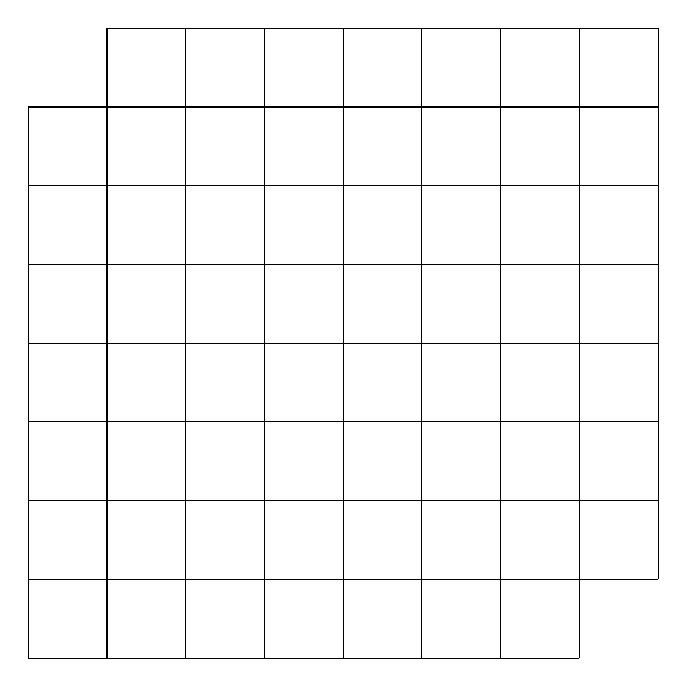
\begin{tikzpicture}
            \draw (0,0) -- (7,0);
            \draw (0,1) -- (8,1);
            \draw (0,2) -- (8,2);
            \draw (0,3) -- (8,3);
            \draw (0,4) -- (8,4);
            \draw (0,5) -- (8,5);
            \draw (0,6) -- (8,6);
            \draw (0,7) -- (8,7);
            \draw (1,8) -- (8,8);
            \draw (0,0) -- (0,7);
            \draw (1,0) -- (1,8);
            \draw (2,0) -- (2,8);
            \draw (3,0) -- (3,8);
            \draw (4,0) -- (4,8);
            \draw (5,0) -- (5,8);
            \draw (6,0) -- (6,8);
            \draw (7,0) -- (7,8);
            \draw (8,1) -- (8,8);
          \end{tikzpicture}
        }
        \captionsetup{labelformat=empty}
        \caption{(a)}
      \end{minipage}
      \(\longrightarrow\)
      \begin{minipage}{0.4\textwidth}
        \centering
        \resizebox{!}{5cm}{
          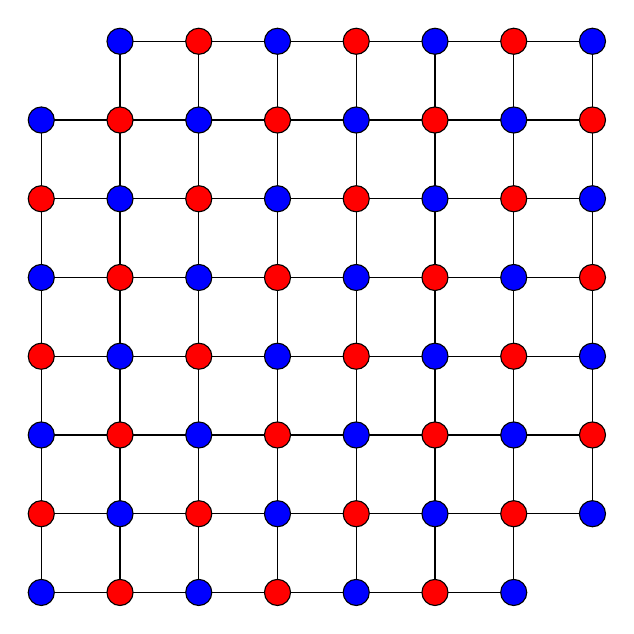
\begin{tikzpicture}[every node/.style={circle,draw}]
            \draw (0,0) -- (6,0);
            \draw (0,1) -- (7,1);
            \draw (0,2) -- (7,2);
            \draw (0,3) -- (7,3);
            \draw (0,4) -- (7,4);
            \draw (0,5) -- (7,5);
            \draw (0,6) -- (7,6);
            \draw (1,7) -- (7,7);
            \draw (0,0) -- (0,6);
            \draw (1,0) -- (1,7);
            \draw (2,0) -- (2,7);
            \draw (3,0) -- (3,7);
            \draw (4,0) -- (4,7);
            \draw (5,0) -- (5,7);
            \draw (6,0) -- (6,7);
            \draw (7,1) -- (7,7);

            \node[fill=blue] at (0,6) {};
            \node[fill=blue] at (1,7) {};
            \node[fill=blue] at (0,4) {};
            \node[fill=blue] at (1,5) {};
            \node[fill=blue] at (2,6) {};
            \node[fill=blue] at (3,7) {};
            \node[fill=blue] at (0,2) {};
            \node[fill=blue] at (1,3) {};
            \node[fill=blue] at (2,4) {};
            \node[fill=blue] at (3,5) {};
            \node[fill=blue] at (4,6) {};
            \node[fill=blue] at (5,7) {};
            \node[fill=blue] at (0,0) {};
            \node[fill=blue] at (1,1) {};
            \node[fill=blue] at (2,2) {};
            \node[fill=blue] at (3,3) {};
            \node[fill=blue] at (4,4) {};
            \node[fill=blue] at (5,5) {};
            \node[fill=blue] at (6,6) {};
            \node[fill=blue] at (7,7) {};
            \node[fill=blue] at (2,0) {};
            \node[fill=blue] at (3,1) {};
            \node[fill=blue] at (4,2) {};
            \node[fill=blue] at (5,3) {};
            \node[fill=blue] at (6,4) {};
            \node[fill=blue] at (7,5) {};
            \node[fill=blue] at (4,0) {};
            \node[fill=blue] at (5,1) {};
            \node[fill=blue] at (6,2) {};
            \node[fill=blue] at (7,3) {};
            \node[fill=blue] at (6,0) {};
            \node[fill=blue] at (7,1) {};

            \node[fill=red] at (0,5) {};
            \node[fill=red] at (1,6) {};
            \node[fill=red] at (2,7) {};
            \node[fill=red] at (0,3) {};
            \node[fill=red] at (1,4) {};
            \node[fill=red] at (2,5) {};
            \node[fill=red] at (3,6) {};
            \node[fill=red] at (4,7) {};
            \node[fill=red] at (0,1) {};
            \node[fill=red] at (1,2) {};
            \node[fill=red] at (2,3) {};
            \node[fill=red] at (3,4) {};
            \node[fill=red] at (4,5) {};
            \node[fill=red] at (5,6) {};
            \node[fill=red] at (6,7) {};
            \node[fill=red] at (1,0) {};
            \node[fill=red] at (2,1) {};
            \node[fill=red] at (3,2) {};
            \node[fill=red] at (4,3) {};
            \node[fill=red] at (5,4) {};
            \node[fill=red] at (6,5) {};
            \node[fill=red] at (7,6) {};
            \node[fill=red] at (3,0) {};
            \node[fill=red] at (4,1) {};
            \node[fill=red] at (5,2) {};
            \node[fill=red] at (6,3) {};
            \node[fill=red] at (7,4) {};
            \node[fill=red] at (5,0) {};
            \node[fill=red] at (6,1) {};
            \node[fill=red] at (7,2) {};
          \end{tikzpicture}
        }
        \captionsetup{labelformat=empty}
        \caption{(b)}
      \end{minipage}
    \end{figure}

      Now, letting \(X\) denote the set of blue vertices, and \(Y\) denote the set of red vertices, it's clear that \(X\) and \(Y\) are independent sets, thus making \(G\) bipartite.  We also have that the neighbor set of \(X\) \(N_G(X) = Y\).

      Since \(|N_G(X)| = |Y| = 30 < 32 = |X|\), we have that \(G\) contains no matching that saturates every vertex in \(X\) directly from theorem 5.2.  In other words, if our board (a) had squares corresponding to the vertex colors in (b), there's no placing of \(1 \times 2\) rectangles such that every blue square is covered by theorem 5.2.
  \end{proof}


  \itm{5.2.4} Let \(A_1, A_2, \hdots, A_m\) be subsets of a set \(S\).  A \textit{system of distinct representatives} for this family is a subset \(\{a_1, a_2, \hdots, a_m\}\) of \(S = \{s_1, s_2, \hdots, s_n\}\) such that \(a_i \in A_i\), \(1 \leq i \leq m\), and \(a_i \neq a_j\) for \(i \neq j\).  Show that \((A_1, A_2, \hdots, A_m)\) has a system of distinct representatives if and only if \(\Big|\bigcup\limits_{i \in J} A_i \Big| \geq |J|\) for all subsets \(J\) of \(\{1,2,\hdots,m\}\). (P. Hall)

    To show this, we will use theorem 5.2 in the book. \n

    \textit{5.2: Let \(G\) be a bipartite graph with bipartition \((X,Y)\).  Then \(G\) contains a matching that saturates every vertex of \(X\) if and only if \(\;|N_G(X')| \geq |X'|\) for all  \(X' \subseteq X.\)}

  \begin{proof}
    We shall prove this by rewording the claim to match the already-proven theorem above. Define \(\F := \{A_1, A_2, \hdots, A_m\}\).  To be a family of subsets of \(S = \{s_1, s_2, \hdots, s_n\}\).  We know there exists a system of distinct representatives (or transversal) if we can find an injective function \(t \colon \F \to S\), with the property that for \(A \in \F\), \(t(A) \in A\) (\(t\) being injective tells us each element in the image is unique).  The image \(t(\F) = \{a_1, a_2, \hdots, a_m\}\) is our actual transversal. \n

    Now instead of thinking of this in terms of sets and mappings, let's instead think in terms of vertex sets and edges.  Let \(G = \left((X \cup Y),E\right)\) be a graph, and define our vertex set \(X := \{x_1, x_2, \hdots, x_m\}\), where each \(x_i\) corresponds to \(A_i \in \F\).  Similarly, define our other vertex set \(Y := \{y_1, y_2, \hdots, y_n\}\), where each \(y_i\) corresponds to \(s_i \in S\).  Finally, we add edges by defining 
    \[E := \{x_iy_j \mid 1 \leq i \leq m, \; 1 \leq j \leq n, \; s_j \in A_i\}.\]

    Clearly, our constructed graph \(G\) is bipartite, as our edges relate sets with elements, and since there are no nested sets or elements inside of elements \(X\) and \(Y\) must both be independent vertex sets.  We can now conclude that \((X,Y)\) is our bipartition. \n

    With all this setup, we can finally apply theorem 5.2.  Since \(G\) bipartite, \(G\) contains a matching that saturates every vertex if and only if \(|N(X')| \geq |X'|\) for all \(X' \subseteq X\). \n
    
    A matching in \(G\) is analogous to a transversal of \(\F\), so \(G\) has a matching that saturates all vertices in \(X\) if and only if \((A_1, A_2, \hdots, A_m)\) has a system of distinct representatives. \n

    \(\Big|\bigcup\limits_{i \in J} A_i \Big| \geq |J|\) for all subsets \(J\) of \(\{1,2,\hdots,m\}\) is analogous to saying that for all \(X' \subseteq X\), the number of distinct vertices adjacent to all the \(x_i \in X'\) is at least as big as the number of vertices in \(X'\), or in other words \(|N_G(X')| \geq |X'|\), which is exactly the right hand side of theorem 5.2. \n

    Now we have the following relation:
    \begin{align*}
      (A_1, A_2, \hdots, A_m) \text{ has a transversal } &\iff \text{ there's a matching that saturates all vertices in } X \\
                                                         &\iff |N_G(X')| \geq |X'| \text{ for all } X' \subseteq X \\
                                                         &\iff \Big|\bigcup\limits_{i \in J} A_i \Big| \geq |J|  \text{ for all } J \subseteq \{1,2,\hdots,m\}
    \end{align*}
    Thus, our claim is proven.
  \end{proof}
  


  \itm{5.2.5} A \textit{line} of a matrix is a row or a column of the matrix.  Show that the minumum number of lines containing all the 1's of a (0,1)-matrix is equal to the maximum number of 1's, no two of which are in the same line.

  \itm{5.5.1} A \textit{diagonal} of an \(n \times n\) matrix is a set of \(n\) entries no two of which belong to the same row or the same column.  The weight of a diagonal is the sum of the entries in it.  Find a minimum-weight diagonal in the following matrix:
  \[\begin{pmatrix}
    4  & 5  & 8  & 10 & 11 \\
    7  & 6  & 5  & 7  & 4  \\
    8  & 5  & 12 & 9  & 6  \\
    6  & 6  & 13 & 10 & 7  \\
    4  & 5  & 7  & 9  & 8  \\
  \end{pmatrix}\]
\end{itemize}
\end{document}
